
\begin{figure*}[t!]
    \centering
    \begin{subfigure}[b]{0.3\textwidth}
    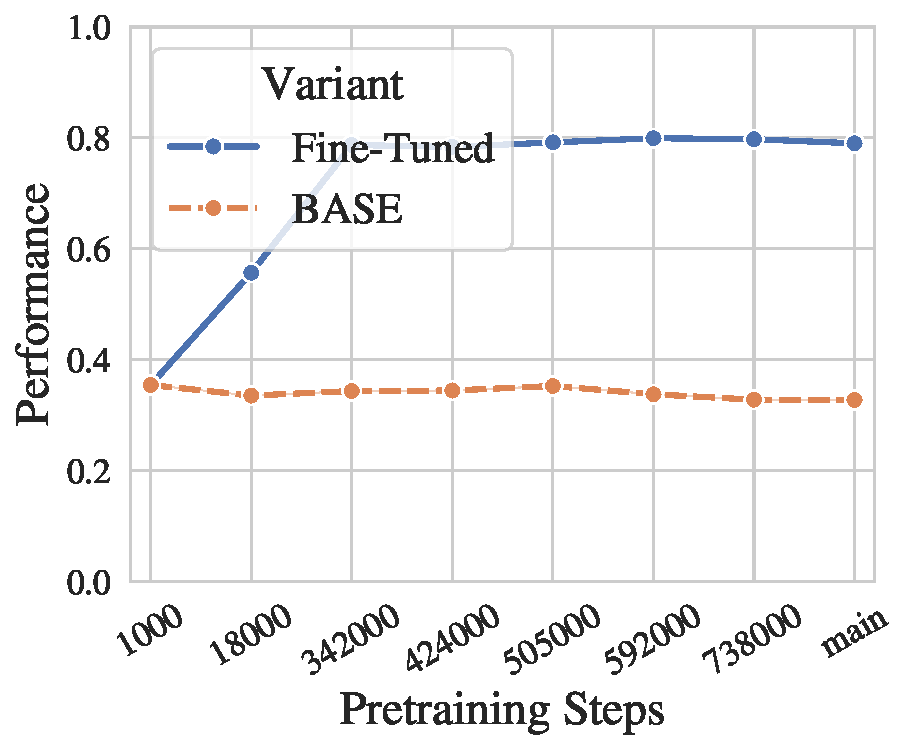
\includegraphics[width=\the\columnwidth]{figures/fig_files/ft_ckpts/sft_evalmnli_matched-trainmnli.pdf}
        \caption{MNLI matched}
    \end{subfigure}%
    ~ 
    \begin{subfigure}[b]{0.3\textwidth}
    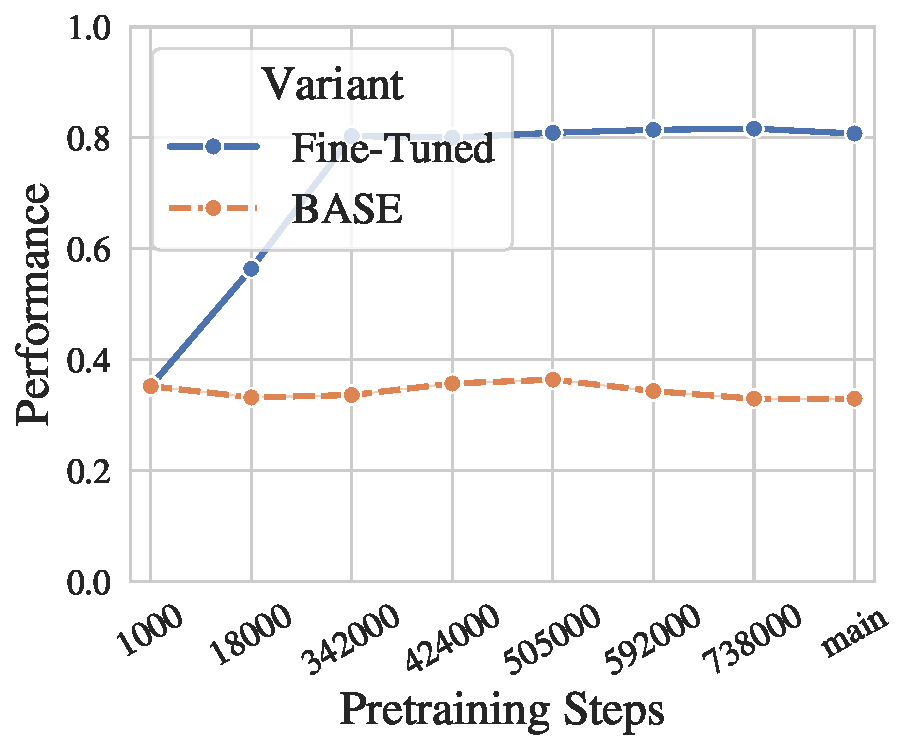
\includegraphics[width=\the\columnwidth]{figures/fig_files/ft_ckpts/sft_evalmnli_mismatched-trainmnli.pdf}
        \caption{MNLI mismatched}
    \end{subfigure}%
    ~ 
    \begin{subfigure}[b]{0.3\textwidth}
    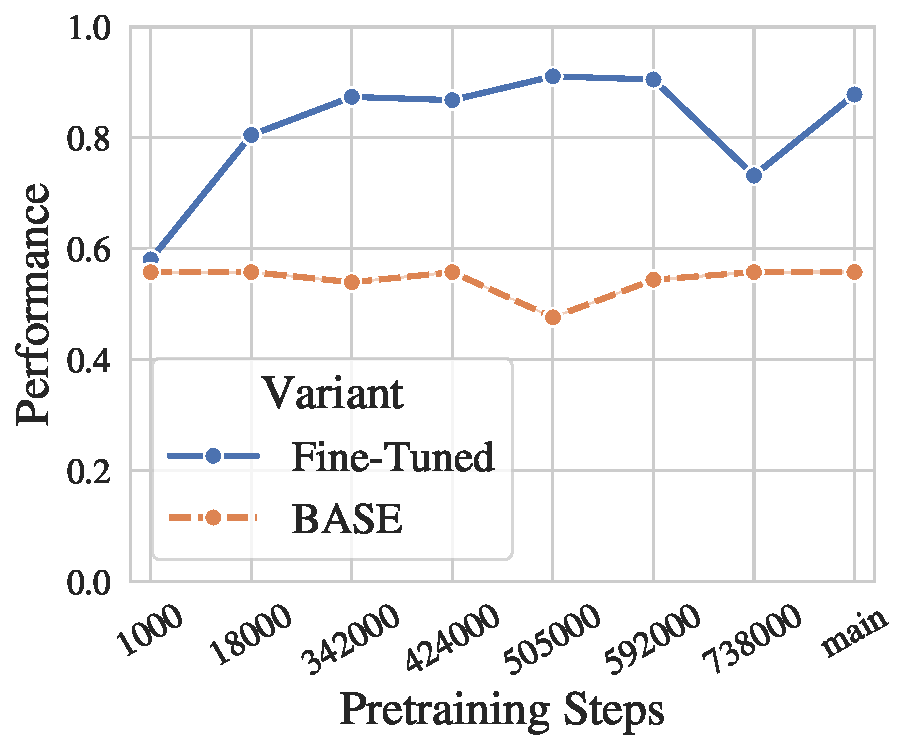
\includegraphics[width=\the\columnwidth]{figures/fig_files/ft_ckpts/sft_evalpaws-trainpaws.pdf}
        \caption{Paws}
    \end{subfigure}%
    \\
    \begin{subfigure}[b]{0.3\textwidth}
    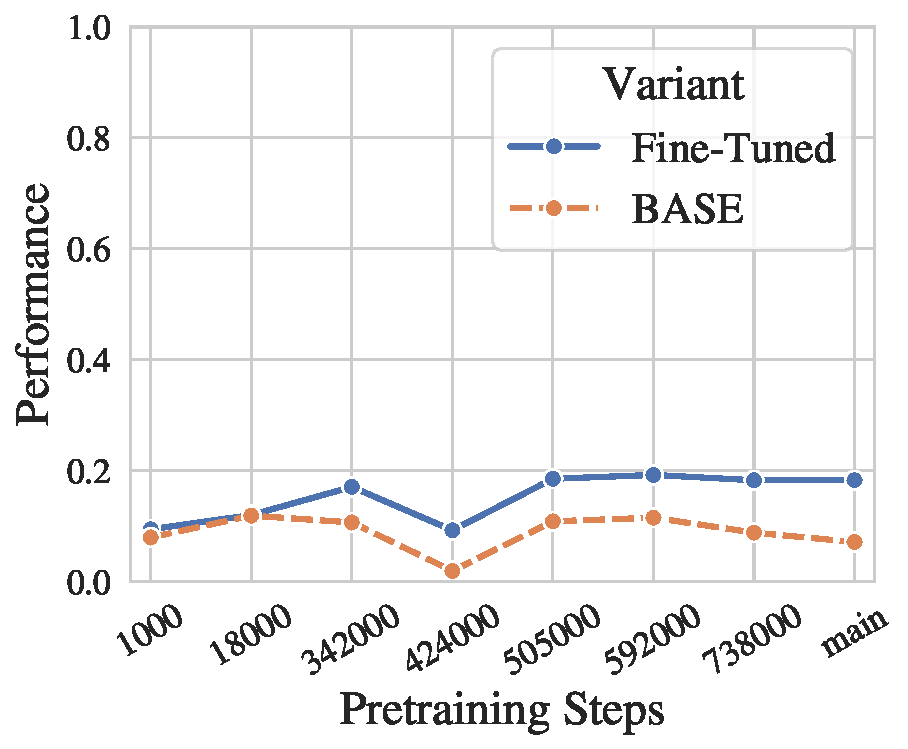
\includegraphics[width=\the\columnwidth]{figures/fig_files/ft_ckpts/sft_evalxsum-trainxsum.pdf}
        \caption{XSum}
    \end{subfigure}%
    ~ 
    \begin{subfigure}[b]{0.3\textwidth}
    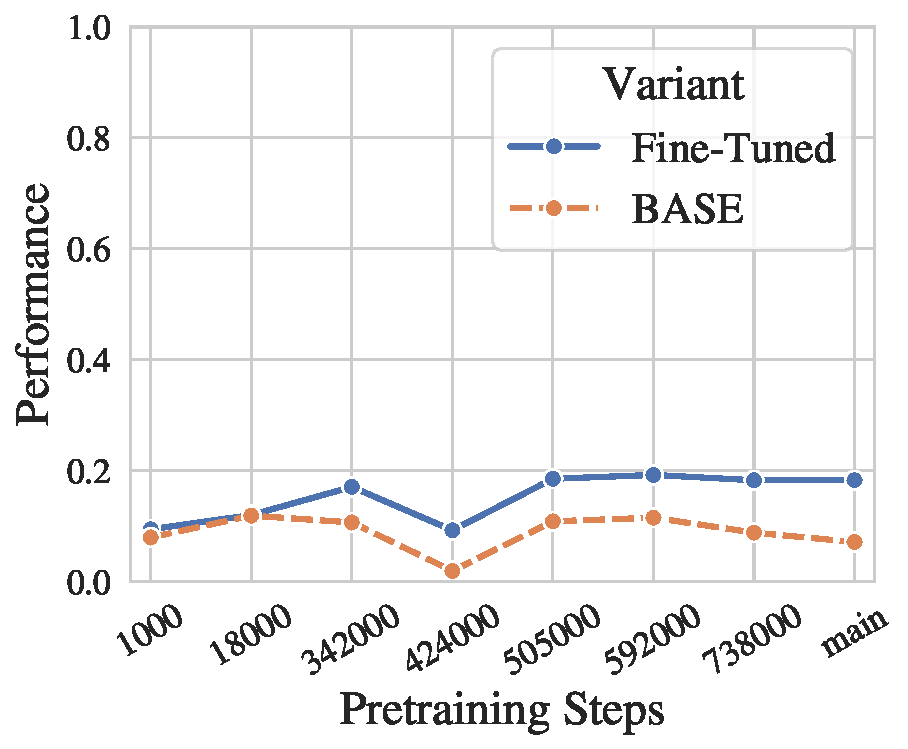
\includegraphics[width=\the\columnwidth]{figures/fig_files/ft_ckpts/sft_evalxsum-trainxsum.pdf}
        \caption{XLSum}
    \end{subfigure}%
    ~ 
    \begin{subfigure}[b]{0.3\textwidth}
    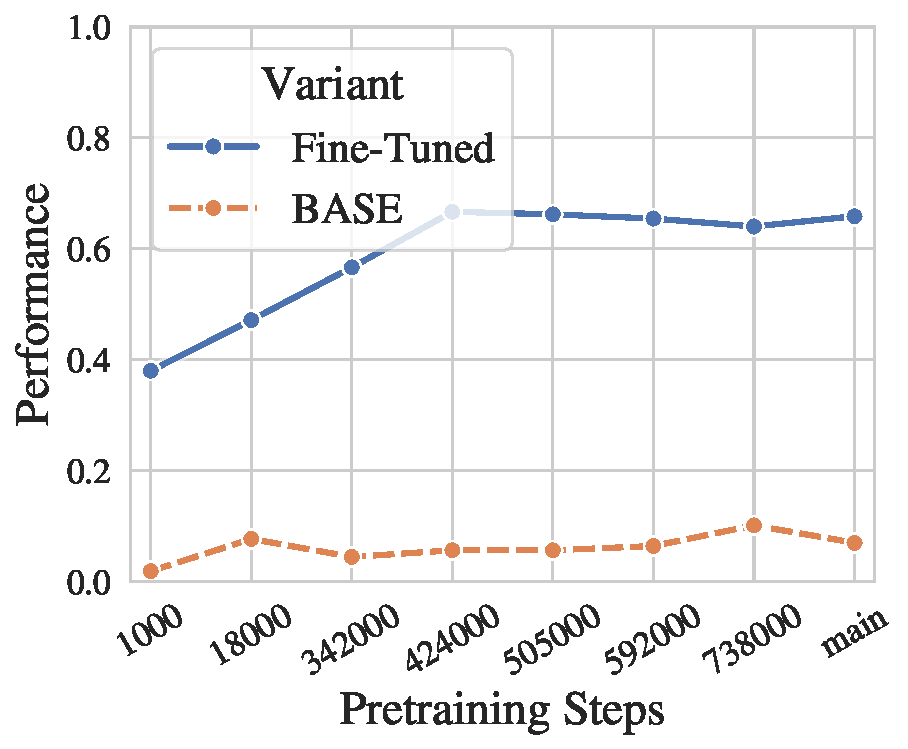
\includegraphics[width=\the\columnwidth]{figures/fig_files/ft_ckpts/sft_evalsocialiqa-trainsocialiqa.pdf}
        \caption{SocialIQA}
    \end{subfigure}%
    \caption{Model performance after supervised fine-tuning on each pre-training step.}
    \label{fig:sft-ckpt-perf}
\end{figure*}